\section{Architecture}

This section covers the architecture of the developed library, primary components and modules, the sequence of operations processing on the GPUs. The library is designed in order to overcome the limitation of the existing solutions, mentioned in the previous section.

\subsection{Design principles}

SPLA library is designed the way to maximize potential library performance, simplify its implementation and extensions, and to provided the end-user verbose, but effective interface allowing customization and precise control over operations execution. These ideas are captured in the following principles.

\begin{itemize}
    \item \textbf{OpenCL API}. The library must use the OpenCL API to accelerate computations on a single OpenCL-compatible GPU device in the system. This API is supported on a variety of graphics accelerators, and also allows you to dynamically compile GPU code at runtime, which saves the user from installing and using a third-party specialized compiler.

    \item \textbf{DAG-based expressions}. The user defines tasks for computations in the form of a directed acyclic graph of expressions, using the library interface to create graph nodes and dependencies between nodes in a declarative style. The user then passes the entire graph to the library for execution, and can either block or wait in a non-blocking way the result.
    
    \item \textbf{User data types}. The library provides the ability to create arbitrary custom types. The type is represented by the unique name and size of the elements in bytes. The elements of the type are POD structures, treated as regular byte sequences.
    
    \item \textbf{User functions}. The library provides the ability to create user-defined functions that can take user-defined (arbitrary) types as input, and which can be used to parameterize mathematical operations. Functions are defined as a set of sinks with OpenCL code, which allows you to create functions without using third-party tools to compile custom code.
    
    \item \textbf{Automated scheduling}. The library automatically splits the expression graph into many tasks and subtasks, which are ordered according to dependencies and distributed to the GPU device. This work is hidden from the user and does not require any action from him.
    
    \item \textbf{Automated hybrid storage format}. The library automatically formats the data, stores it in a hybrid format, and distributes it automatically between the computing device and the host. This work, storage format, distribution details are hidden from the user and do not require any action from him.
    
    \item \textbf{Exportable interface}. The library has a C++ interface with an automated reference-counting and with no-templates usage. It can be wrapped by C99 compatible API and exported to other languages, for example, in a form of a Python package.
\end{itemize}

\subsection{Execution model}

The general idea of the library expression execution is depicted in the figure~\ref{fig:execution_schema}.

As an input library accepts the expression in a form of DAG. The DAG is created using library API. Vertices of the computational graph are the fundamental operations, which process primitives such as matrices or vectors. This operations can read or write data, compute product, etc. Directed edges between vertices show data dependencies between operations. If the edge is present between operations, then the next operation is executed only after the previous one is fully finished. This approach allows to specify, which operations must be ordered and which one can be executed in parallel, what allows better occupy the GPU device.

\begin{figure}[ht]
    \centering
    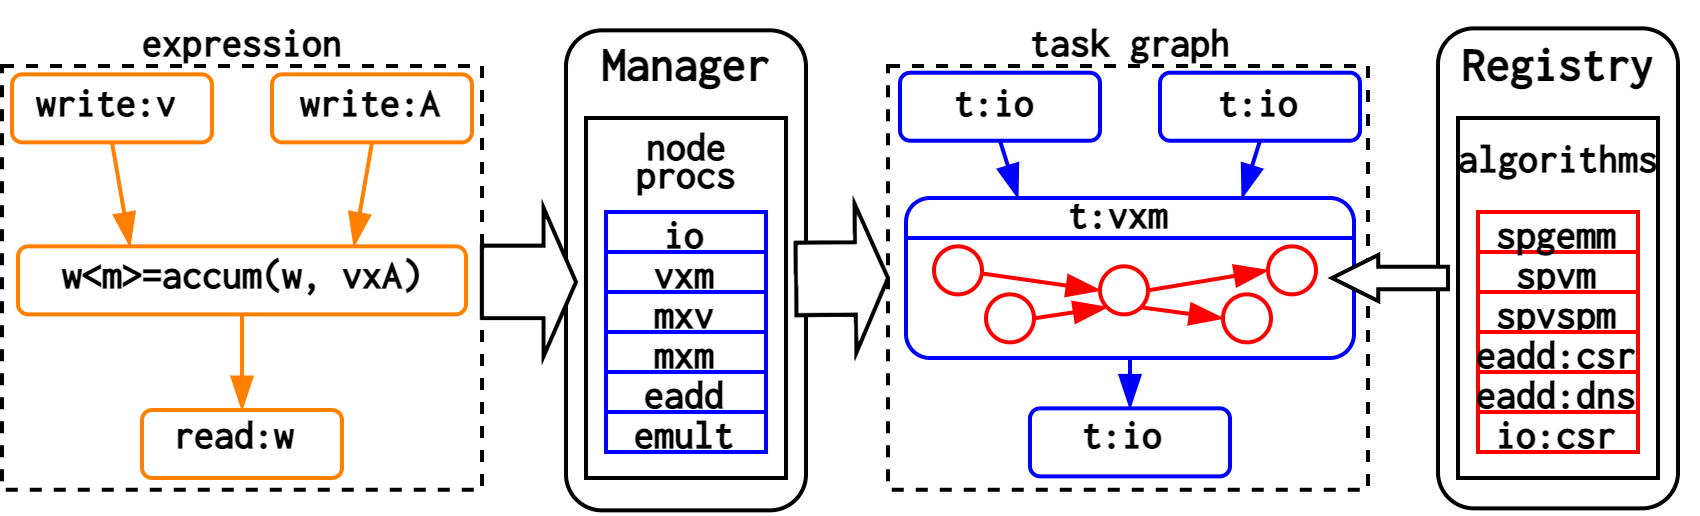
\includegraphics[width=1.0\textwidth]{images/execution_schema.png}
    \caption{Library expression processing schema.}
    \label{fig:execution_schema}
\end{figure}

The DAG expression is submitted to the library for the execution. The expression is traversed and for each a specialized processor is found. The processor is responsible for a processing of a single node. It is possible to have multiple processors for a single type operations with specialized rules of selection. This approach allows to separate the data and the execution, as well as gives an ability to handle some edge cases and optimize operation for a particular set of input arguments.

Processors are used to construct a task graph from the expression. Each processor adds tasks and subtasks for the execution of a particular node. External dependencies between nodes are preserved and translated into dependencies between tasks. Dependencies between subtasks inside a single task are defined by a node processor. 

Subtasks are spawned regardless of the storage format and parameters of a particular input arguments. For each type of the arguments there may be present a specialized algorithm in the registry. Algorithm is selected automatically at runtime using a set of rules and priorities. It is possible to specialize algorithm for any type of format and register them without processor code modification. 

The task graph is scheduled a whole object to the execution on a multi-core GPU in a multi-threaded mode. CPU threads process tasks and subtasks in a safe manner, since all data dependencies are preserved due to the nature of submitted DAG expression. Each subtask uses separate GPU scheduling queue, so it offloads the GPU with a work without serialization.

Expressions are executed asynchronously. The user after submission gets a special \textit{future} object, which allows either to block until completion or to probe the state of the expression in a non-blocking fashion.

\subsection{Data Storage}

\begin{figure}
    \centering
    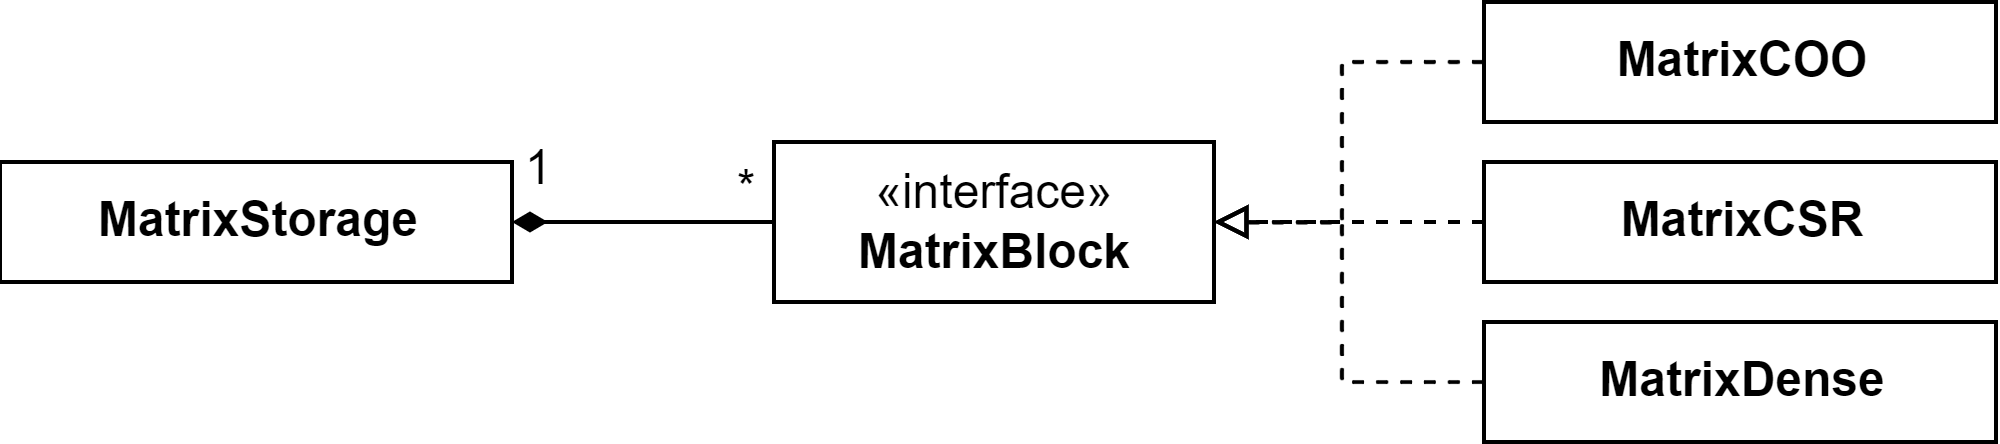
\includegraphics[width=0.9\textwidth]{images/matrix_storage_hie.png}
    \caption{Class hierarchy for matrix storage.}
    \label{fig:matrix_storage_hie}
\end{figure}

Library provides hybrid blocked storage format for matrix and vector representation in CPU and device memory. The idea of the concept is depicted in the diagram~\ref{fig:matrix_storage_hie}. Blocked storage usage allows provides following benefits.

\begin{itemize}
    \item Allows to precisely select format depending on the density of the section of the matrix.
    \item Allows to utilize multiple algorithms to multiply primitives.
    \item Allows to offload part of the matrix or vector from GPU memory to save a space.
\end{itemize}

Matrix storage class is responsible for managing the data of the matrix object. Each matrix instance has its matrix storage class. Storage represents a set of matrix blocks with unified interface, where each block may have a specialised implementation with support for a particular data format, such as \textit{list of coordinates} (COO), \textit{compressed sparse rows} (CSR), \textit{dense}, etc. The list of possible formats is not limited by the design of the library.

For example purposes only, consider \textbf{3x4} matrix storage grid as depicted in the figure~\ref{fig:blocked_mxv}. Blocks form the one or two dimensional grid. The grid is divided into a series of square blocks of equal size except edge blocks, which has clamped size to the matrix dimensions. Each block has unique storage format. Empty blocks not stored in the storage. They do not consume any resources. Size of the block is defined by a constant at library start up. In the extreme case, this constant can be set to \textit{inf}, so the grid will always has \textbf{1x1} size.

Multiplication process of object with such a grid schema is straightforward and is done using blocked multiplication. It is guaranteed that matrix and vector with compatible dimensions will always have compatible grid properties.

\begin{figure}
    \centering
    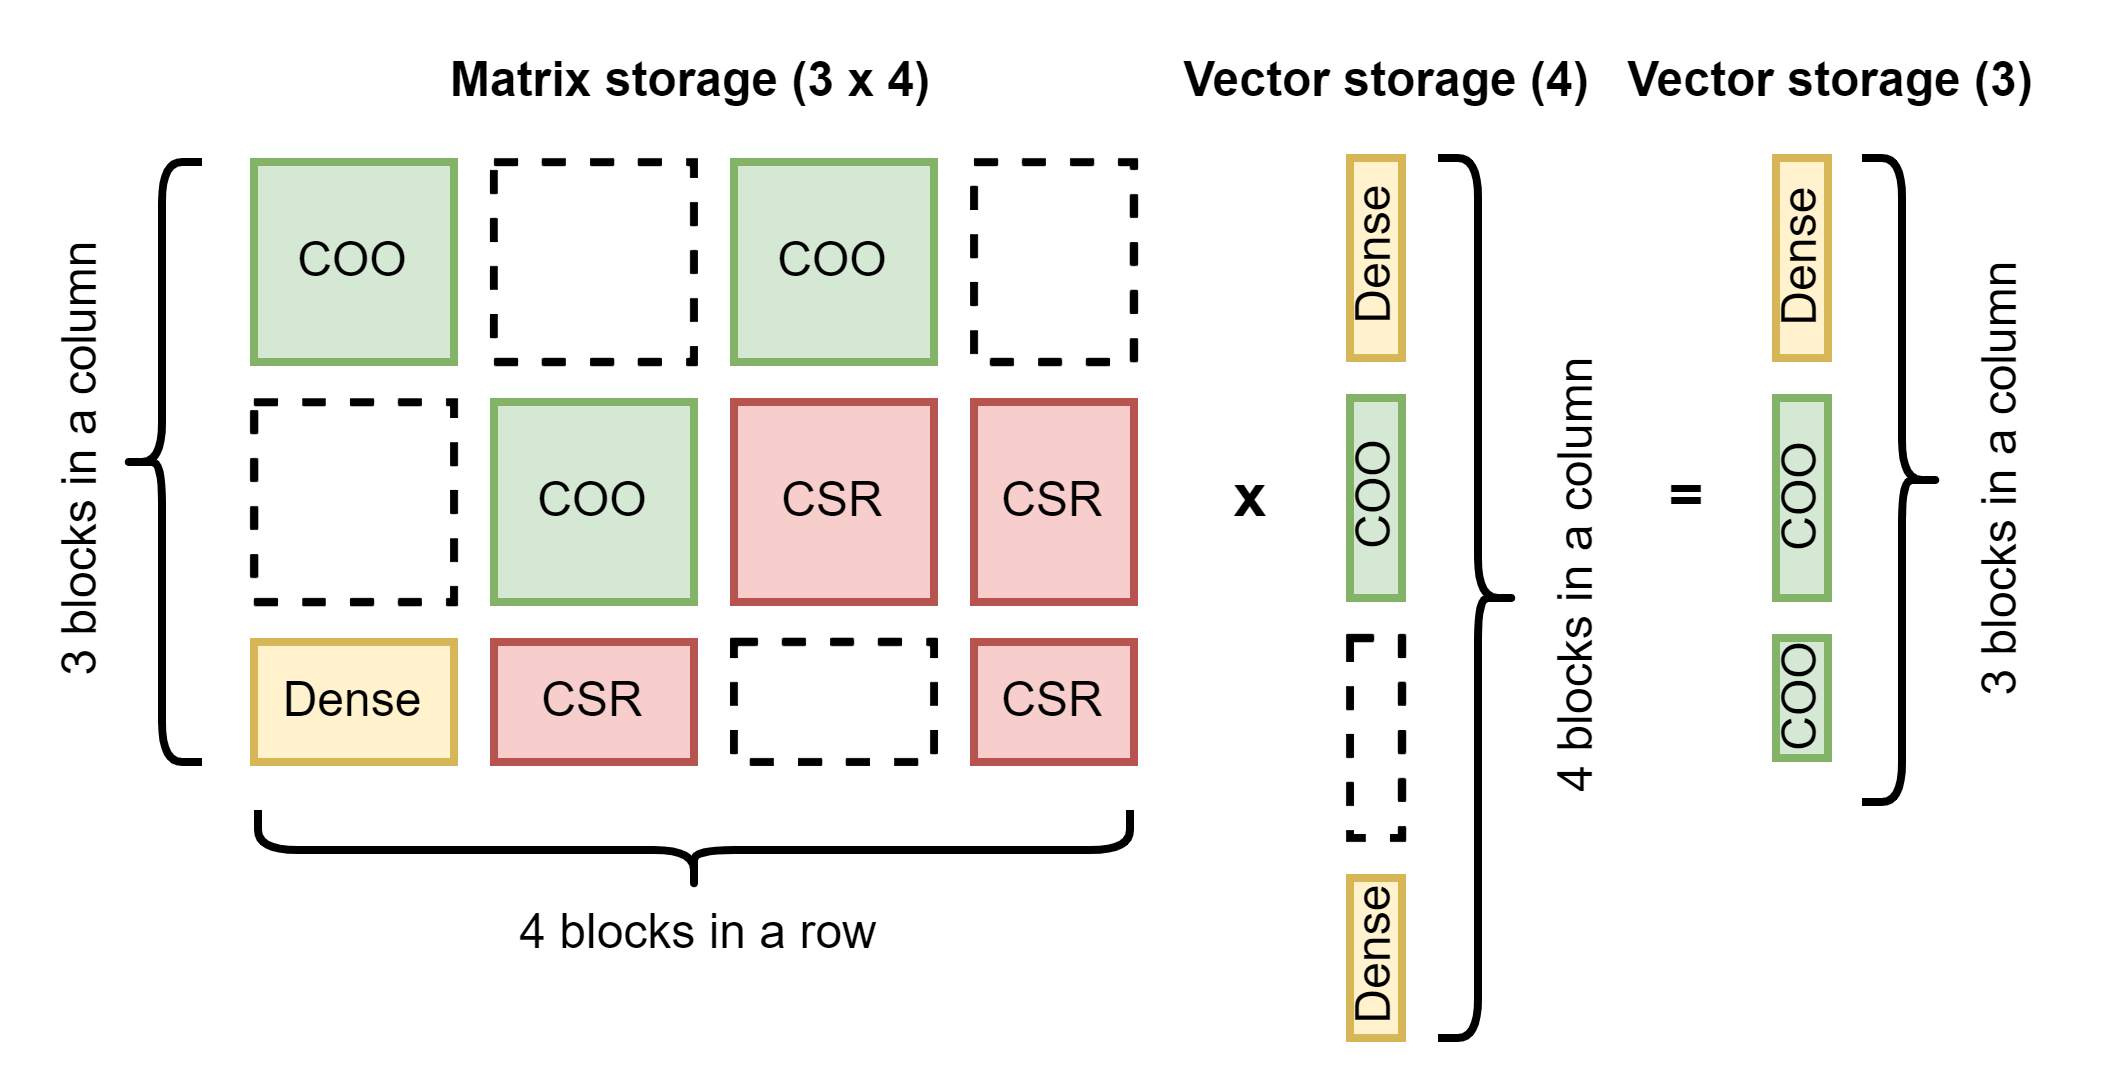
\includegraphics[width=0.9\textwidth]{images/blocked_storage_mxv.png}
    \caption{Blocked storage based matrix-vector product.}
    \label{fig:blocked_mxv}
\end{figure}

\subsection{Algorithms registry}

As it was mentioned in the previous section, matrix and vector containers may be stored in a number of storage formats. Thus, it is important to support operations for all particular cases. Library segregates the particular algorithm invocation and its particular implementation. It provides the following features.

\begin{itemize}
    \item Allows to invoke the operation without knowledge about underlying storage format.
    \item Allows to select the algorithm for a particular set of input parameters with a particular storage format at runtime, where extra information is available.
    \item Allows to extend the library algorithms and formats support without modification of the existing source code.
    \item Allows to treat blocks of matrix and vector grids as ordinary objects, so it is possible to write generalized blocked products.
\end{itemize}

\begin{figure}
    \centering
    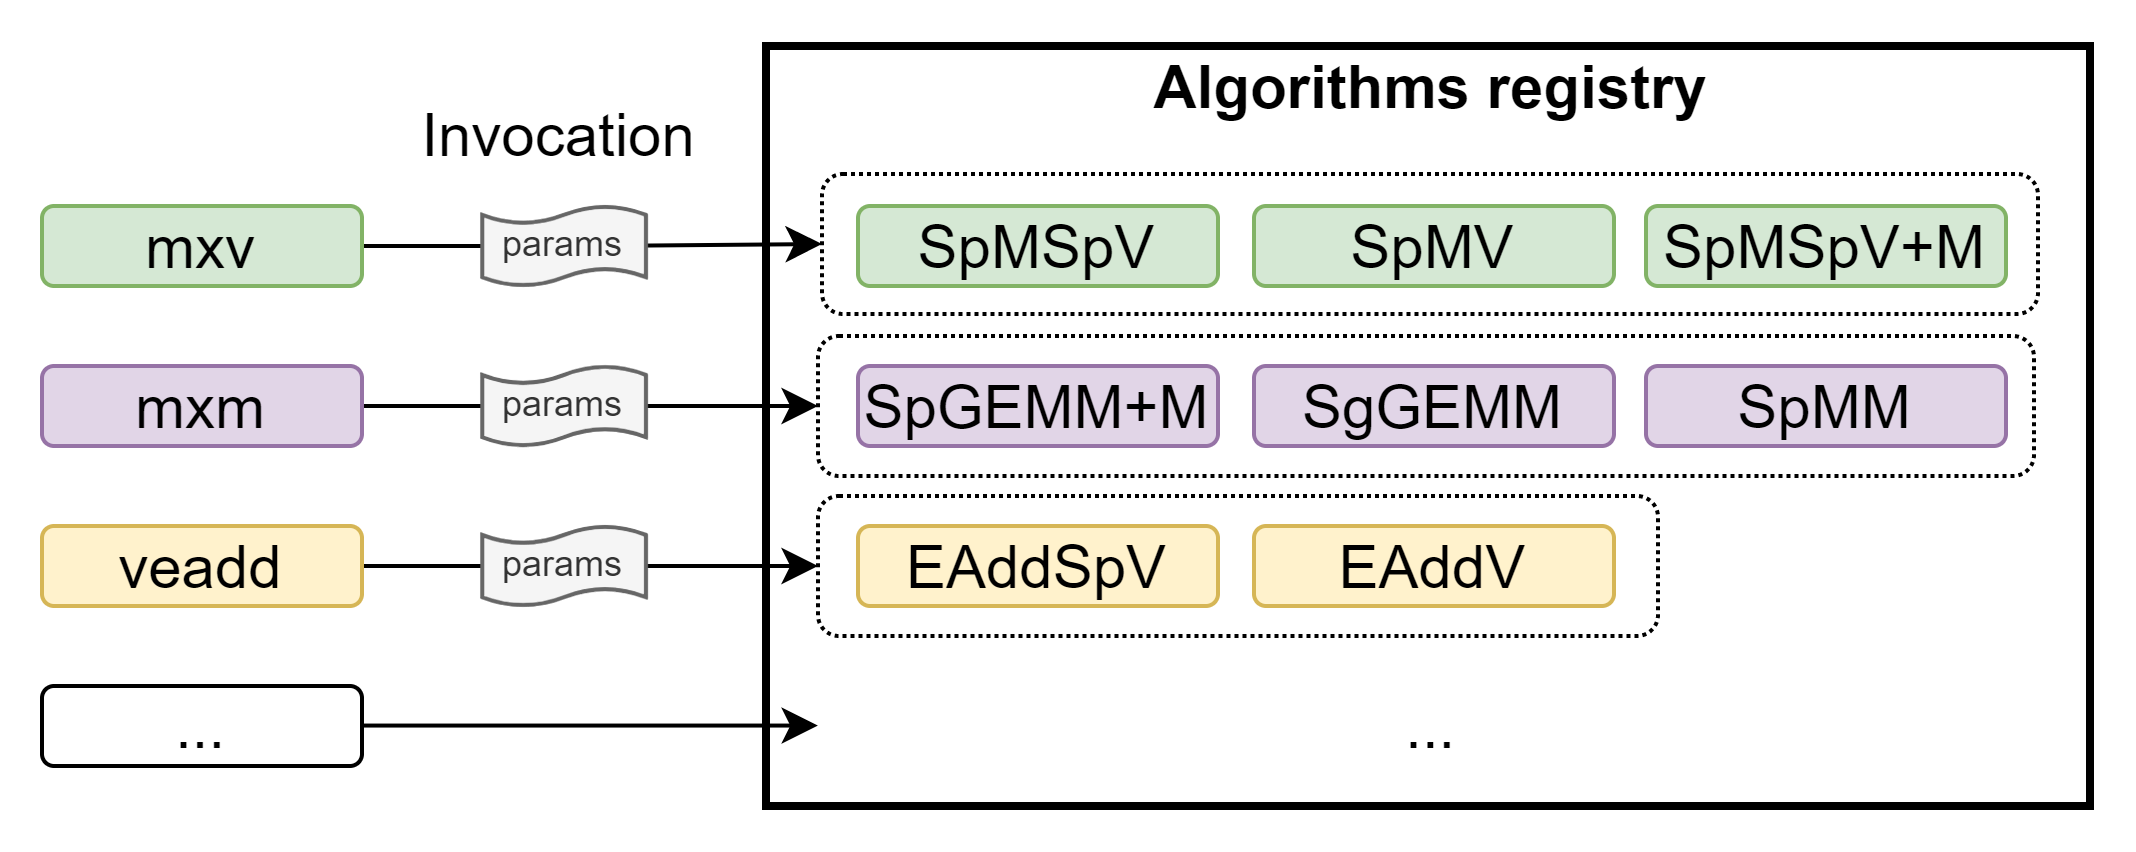
\includegraphics[width=0.9\textwidth]{images/algo_registry_idea.png}
    \caption{Idea of algorithm invocation segregation.}
    \label{fig:algo_reg_idea}
\end{figure}

The idea of the invocation segregation is depicted in the figure~\ref{fig:algo_reg_idea}. For example, consider matrix-vector product. When we want to multiply some matrix block by some vector block, we use \textit{mxv} operation. For the invocation we pack params and send them to the algorithms registry. Registry is responsible for the selection of the best suitable implementation for the evaluation.

More details about this mechanism are provided in the partial class diagram~\ref{fig:algo_reg_classes}. For the invocation the generalized \textit{AlgoParams} structure is provided. It stores id of the device for the execution and the descriptor with extra parameters to control evaluation. This structure is sub-classed by particular algorithms to add extra parameters, required for algorithms evaluation. The \textit{Algo} interface provides unified functionality, required to store, select and invoke a particular algorithm.

The library relies on the C++ runtime type information, to distinguish parameters structures for different algorithms. Particular algorithms implementations are stored in the registry class in the order of registration. The selection is order based, so the first best fitting algorithm is selected for the execution. This mechanism can be changed in the future with modification of the \textit{AlgoRegistry} class only.

\begin{figure}
    \centering
    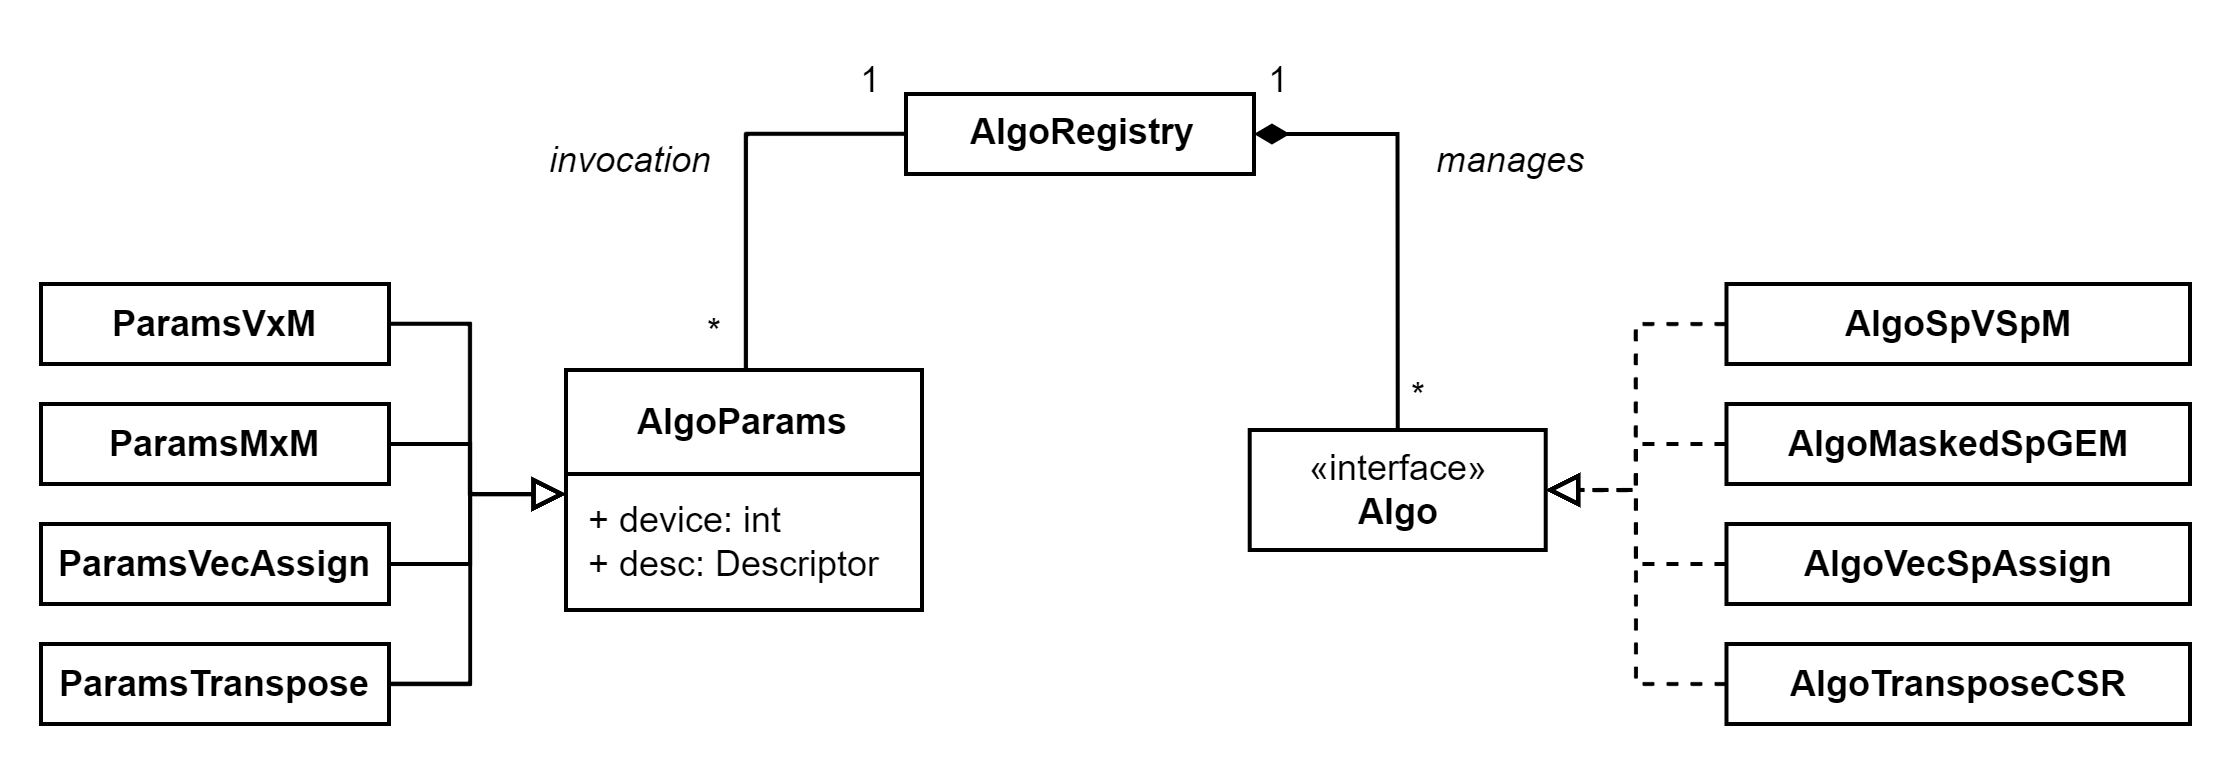
\includegraphics[width=1.0\textwidth]{images/algo_registry_classes.png}
    \caption{Class hierarchy for algorithms registry.}
    \label{fig:algo_reg_classes}
\end{figure}